\chapter{Algorithm Implementation}
This chapter deals with the implementation-specific details of the algorithms. Specifically the chapter will discuss how the intermediate features and main features are implemented such that they can be evaluated in a smart-phone environment. This is important because it cannot be taken for granted that data can be stored without thinking of how to do this in a smart manner. In addition many of the features cannot be directly implemented according to their mathematical definition provided in Chapter \ref{chapter:03-design}. This is due to Dart being an imperative programming language which does not support mathematical and vector notation, such as is the case with scripting language such as Python and MATLAB. 

Intermediate features are extracted from sequences of location samples by applying the following algorithm. To identify stops, location samples are traversed sequentially and grouped according to a maximum distance threshold. If a sample is too far from the current group median location, a new group is formed. Initially this strategy creates a lot of groups, which are then filtered by a minimum duration threshold leaving groups where movement stopped for at least some time. Each remaining group represents a stop, described by the median coordinates of the group of location samples and arrival and departure time based on the first and last location sample in the group. The appropriate values of maximum distance and minimum duration depends on the accuracy and sample frequency of the data. We applied a minimum distance of 50 meters and minimum duration of 20 minutes based on inspecting the distributions of distances and times between subsequent location samples in the dataset.

As an intermediate step, stops that are close in terms of time and distance and have no other stops in between are merged to reduce noise caused by outlier location samples that might break a stop into several stops. We merged stops that were maximum 5 minutes and 5 meters apart and found that this removed cases with a suspicious amount of stops per day. With the stops available, places are identified by clustering stops using the DBSCAN clustering algorithm [Ester et al. 1996] with a minimum cluster size of 1, effectively identifying stops appearing at the same location. Each place is represented by the median coordinates of the included stops along with a unique place ID. The place ID is also appended to each of the included stops associating each stop with a place. We applied a maximum distance of 50 meters between stops when computing the clusters.

Moves where identified by selecting the sequences of location samples in between stops. Each move is described by departure and arrival time based on the first and last location sample in the sequence, the origin and destination place ID and the total distance between the location samples in the sequence. The moves were filtered by a minimum duration and minimum distance. We applied a minimum duration of 5 minutes and a minimum distance of 50 meters. Daily features derived from the stops, places and moves include stops count, stops total duration, places count, moves count, moves total distance and moves total duration.

\begin{minted}{python}
collect_data_continuously()
on data_point:
	save_to_disk(data_point)
	if trigger:
        points = load_todays_data_from_disk()
		stops_hist, moves_hist = load_from_disk()
		stops = stops_hist + find_stops(points)
		moves = moves_hist + find_moves(stops, points)
		features = feature_extraction(stops, places, moves)
		# do something with the features
		save_to_disk(stops, moves)
\end{minted}

\subsection{Feature Extraction}
The feature extraction takes place after the data collection and pre-processing has been done, and will use the Stops, Places and Moves to derive the features described in Chapter ??. 

\subsubsection{Number of Clusters}
Defined as the number of non-negative place labels found by the Places algorithm.

\begin{minted}{python}
def num_clusters(places):
    return len(places > 0)
\end{minted}

\subsubsection{Location Variance (LV)} 
LV was computed as the natural logarithm of the sum of the statistical variances of the latitude and the longitude components of the location data. The dataset must contain at least 2 observations to calculate the variance, otherwise the variance of both the latitude- and the longitude will be zero, and thus $LV = log(0 + 0 + 1)  = 0$

\begin{minted}{python}
def location_variance(dataset):
    return log(var(dataset.lat) + var(dataset.lon.var) + 1)
\end{minted}

\subsubsection{Location Entropy (LE)} 
Here, we use the duration spent at each place, found in the duration column in the places dataframe.

\begin{minted}{python}
def entropy(places):
    p = places.duration / sum(places.duration)
    return -sum(p * log(p))
\end{minted}

\subsubsection{Normalized LE} 
Here we just divide LE by the log to the number of places.

\begin{minted}{python}
def normalized_entropy(places):
    return entropy(places) / log(places.length)
\end{minted}

\subsubsection{Time-distribution Table}
The time distribution table tells the story of which places were visited for how long during the day and does this by dividing the day into 24 one-hour time slots represented by rows, and the columns representing the different significant places found by the pre-processing algorithms. Each entry $T[i,j]$ is the number of hours spent at timeslot $i$ at place $j$, which means that the row can maximally sum to 1.0. If the user moves between two places, the row will however not sum to 1.0 since there was time spent at none of the places.

Using the stops, the time spent at each place can be calculated for each hourly timeslot during the day. Concretely, this is done by iterating through each stop and incrementing the time at entry $i,j$ using the arrival time of the stop \verb|1 - row.arrival.minute / 60| by using the \verb|arrival.hour| as the hour slot. For the last time slot the same is done, but using the departure time \verb|row.departure.minute / 60|. Every time slot in between for the the place $j$ is set to 1.0 since the user was there for the full time slot.

\begin{minted}{python}
def make_hour_matrix(stops, num_places):
    h = np.zeros((HOURS_IN_A_DAY, num_places))
    
    for index, row in stops.iterrows():
        pid = row.place
        start_hour = row.arrival.hour
        end_hour   = row.departure.hour
        
        # If user arrived and departed within the same hour
        # Then the time stayed is the diff between departure and arrival
        if start_hour == end_hour:
            h[start_hour, pid] = row.departure.minute - row.arrival.minute
        
        else:
            # Arrival hour
            h[start_hour, pid] = 60 - row.arrival.minute

            # In between
            for hour in range(start_hour+1, end_hour):
                h[hour, pid] = 60

            # Departure hour
            h[end_hour, pid] = row.departure.minute
        
    return h / 60 # Normalize by 60 mins
\end{minted}

\begin{figure}
    \centering
    \begin{tabular}{|l|l|l|l|l|}
    \hline
    \textbf{}        & \textbf{Place \#0} & \textbf{Place \#1} & \textbf{...} & \textbf{Place \#n} \\ \hline
    \textbf{00 - 01} &                    &                    &              &                    \\ \hline
    \textbf{01 - 02} &                    &                    &              &                    \\ \hline
    \textbf{...}     &                    &                    &              &                    \\ \hline
    \textbf{16 - 17} &                    &                    &              &                    \\ \hline
    \textbf{17 - 18} &                    &                    &              &                    \\ \hline
    \textbf{18 - 19} &                    &                    &              &                    \\ \hline
    \textbf{...}     &                    &                    &              &                    \\ \hline
    \textbf{23 - 00} &                    &                    &              &                    \\ \hline
    \end{tabular}
    \caption{Time-place distribution table.}
    \label{fig:time-table}
\end{figure}

\subsubsection{Home Stay} 
The percentage of time the participant has been home place, home being the most visited cluster between 12 am and 6 am which can be identified by using the mean of the the historical time distribution tables, i.e. the place which, on average, was the most visited between 00 and 06 am. Afterwards, all the stops during the day are iterated and the duration of the stops belonging to the home cluster are summed up.

\subsubsection{Transition Time} 
To calculate the transition time of the user the Moves are used, and the difference is time stamps between all the individual data points which make up each move are summed together. 

\subsubsection{Total Distance} 
Same procedure as transition time, except for using the the distances between all the individual data points rather than the duration.

\subsubsection{Routine Index} 
The Routine Index is the RMSE of today's time distribution table compared the historical table, which is the average of all historical tables. The historical tables are computed by loading all historical stops from the disk, and calculating the tables from these. The routine index is always calculated based on the current hour of the day, i.e. at 14:00 only the time-slots from 00:00 to 14:00 are compared to the historical average, between 00:00 and 14:00. 

\begin{minted}{python}
def RI(m, h, end_hour=24):
    if m.sum() == 0:
        # no routine index could be calculated
        return -1.0 
    return 1 - np.abs(m[:end_hour] - h[:end_hour]).mean()
\end{minted}

\begin{figure}
    \centering
    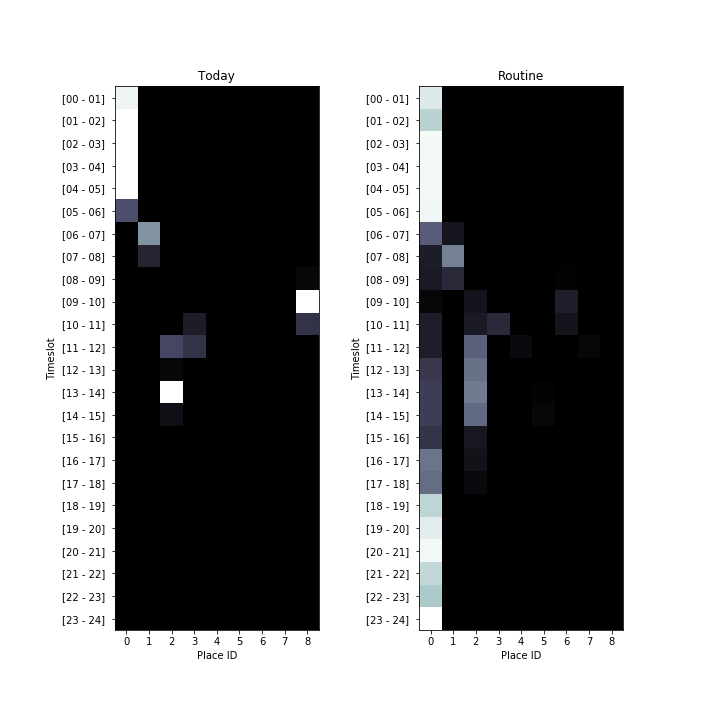
\includegraphics[width=\textwidth]{images/routine.png}
    \caption{An hour matrix of a specific day compared to the Routine Matrix derived from several days of data.}
    \label{fig:routine_example}
\end{figure}

\section{Storing Objects on the Device}
It was necessary to store Stops and Moves on the device, such that which rely on historic data can be computed in the future. For a single day it is also necessary to store all the data points collected on that day, on the disk, in order to minimize the risk of data loss. This was done by defining a buffer of data points which collects all incoming GPS data, and once a certain capacity is reached the data contained in the buffer is written to the disk, and the buffer is emptied.

\subsection{Serialization}
In order to save the SingleLocationPoints from today and historical Stops and Moves on the device they must be transformed from Dart objects into a data format which can store the state of the object, i.e. the information contained within it. The process of doing so is serialization and in this case Dart objects were transformed into JavaScript Object Notation (JSON) objects, which is a very common, human-readable data format that uses key-value pairs to store data. A JSON object can be stored in a database, or it can be transformed to a string in order to be stored. It was chosen to simply transform JSON objects to a string and write them to a local file, rather than storing the information in a database on the phone. The database approach is more involved and was therefore not chosen given the small scope of the project and working from a philosophy of getting a prototype up and running as fast as possible.

JSON supports a limited number of data types, such as strings, numbers, booleans, arrays, objects and null values. This means that in order to translate a Dart object to JSON, all of its fields must be serializable. An example of where this quickly becomes a problem, is with objects such as DateTime objects, since they are not supported by JSON - however a DateTime can be transformed to a number, which is milliseconds since epoch, or to an ISO standard date string. The approach is therefore to look at all the fields of the object that is to be serialized, and ensure that types of these fields all support some form of serialization. If they do not, it must be implemented.

\begin{figure}
    \centering
\begin{minted}{json}
{
    "location": {
        "latitude": 55.11787166161895,
        "longitude": 14.703046919371356
        },
    "datetime": "1586527196999"
}
\end{minted}
    \caption{Example of a serialized SingleLocationDataPoint}
    \label{fig:serialized_point}
\end{figure}

\begin{figure}
    \centering
\begin{minted}{json}
{
    "centroid": {
        "latitude": 55.11787908183754,
        "longitude": 14.703028176721789
        },
    "place_id": 0,
    "arrival": 1586556000999,
    "departure": 1586556697999
}
\end{minted}
    \caption{Example of a serialized Stop}
    \label{fig:serialized_stop}
\end{figure}

\begin{figure}
    \centering
\begin{minted}{json}
{
    "stop_from": {
        "centroid": {
            "latitude": 55.11053332998761,
            "longitude": 14.712282829580444
            },
        "place_id": 6,
        "arrival": 1586694154999,
        "departure": 1586696052001
    },
    "stop_to": {
        "centroid": {
            "latitude": 55.11793063393585,
            "longitude": 14.702982994031046
        },
        "place_id": 0,
        "arrival": 1586697230006,
        "departure": 1586699246824
    },
    "distance":2357.3408321427805
}
\end{minted}
    \caption{Example of a serialized Move}
    \label{fig:serialized_move}
\end{figure}


For loading an object from disk into application memory again it must also support de-serialization which reads values of the JSON object's keys and stores them in a Dart object. If we continue the example of a DateTime object which was serialized by either converting it to a number or a string, de-serialization must use a parser which reads the string bit by bit or use some math for calculating what day a time delta from January 1st 1970 is. 

Serialization and de-serialization is implemented by making an abstract class called Serializable, which has two functions: toJson and fromJson. The toJson function converts the object itself to a JSON object and the fromJson function is a so-called factory function which is in essence a constructor which creates a Dart object given a JSON object. The SingleLocationPoint, Stop and Move classes all implement the Serializable interface, which requires the classes to have a concrete implementation of these two methods, which in turn ensures the compiler that all of these classes can be serialized and de-serialized, which makes generalizing about objects belonging to either of these classes easier. Concretely, a generic class, Serializer<E>, was implemented in order to handle serialization, in which a type E is specified, which must a Serializable class. This makes it efficient in terms of lines of code to serialize a list of objects, since they are all required to implement toJson method, which produces a JSON object, and for de-serialization purposes they can all be constructed from a JSON object, given that it contains a set of correctly formatted key-value pairs.


\section{Unit Testing}
Mostly the model as well as read/writes to local files i.e. Serialization. 
\section{Tuning Parameters}
Parameter tuning was done by taking a few different examples where ground truth is  known, i.e. by having done it myself. The examples include whole days in Munich (GER), Copenhagen (DK) and Bornholm (DK) which all have vastly different environments and acitivties, with Munich having places displaced very far away and where public transporation was necessary. In Copenhagen I travelled by foot, either walking or running and on Bornholm I would travel in the city of Rønne by foot, again walking or running, or going to the other side of the island by car, and walking the dog. Since the ground truth is known for each of these examples, the parameter tuning is done by taking the parameters with the biggest impact such as stop duration and place radius, starting high and then lowering the parameter value until a reasonable result is achieved across the board.
